\section{Electrons and Muons}
\label{sec:leptons}

Electrons and muons, being charged particles, leave identifiable tracks
within the ID.
As a result, their reconstruction involves the use of the tracks and
vertices described in the previous section, using them essentially as initial
seeds for their complete reconstruction.
Electron reconstruction, described in Section~\ref{sec:electrons}, complements the track information provided by the ID
with calorimetric information provided by the EM calorimeter (Section~\ref{sec:calo_em})
and with knowledge about the pattern of transition radiation expected to occur
in the TRT as a result of passing electrons.
Muon reconstruction, described in Section~\ref{sec:muons}, revolves around stitching together the tracks reconstructed
in the ID with those tracks independently reconstructed in the MS layers at large radii.

\subsection{Electrons}
\label{sec:electrons}

\subsubsection{Electron Reconstruction}
\label{sec:electron_reco}

{\color{red}{After 2016 they replaced sliding window algorithm with supercluster-based reco}}

The reconstruction of electron candidates is based on three components which
characterise the signature of electrons: localised clusters of energy
deposits found within the EM calorimeter, charged-particle tracks
identified in the ID, close-matching (in ($\eta,\phi$)) of the tracks to the clusters
that form the final electron candidates~\cite{Aad:2019tso}.
It is generally possible to match multiple tracks to the same electrogmagnetic cluster,
all originating from the same primary electron produced in the hard-scatter.
This is due to the fact that electrons lose significant amounts of energy to bremsstrahlung
photons as they interact with and traverse the ID.
These radiated photons can then undergo conversion to electron-positron pairs,
which, too, can undergo further bremsstrahlung.
The positrons, electrons, and photons are usually emitted in a very collimated fashion
and thus deposit most of their energy in a localised fashion within the calorimter.

The search for localised energy deposits in the EM calorimeter is performed
by following a sliding window algorithm over the individual cells whose dimensions are
defined by the second sampling layer of the EM calorimeter (Figure~\ref{fig:em_calo_section}).
Electron candidates are seeded by localised energy deposits whose summed transverse energy,
across all layers of the EM calorimeter, is greater than $2.5\,\GeV$~\cite{Aad:2019tso}.
These clusters act as seeds for the matching of reconstructed ID tracks.
The reconstructed tracks are refit using a Gaussian Sum Filter (GSF) method~\cite{ATLAS-CONF-2012-047} 
that accurately accounts for the bremsstrahlung energy losses characteristic of
electron traversal and are then matched to the localised clusters using
the cluster barycenter as the point of reference to match in $\eta-\phi$.
If there is no GSF-track candidate matching to the EM calorimeter cluster seed, then
the cluster is marked as an unconverted photon. The cluster is marked as a
converted photon if a matched GSF-track candidate exists but is not associated
with the primary hard-scatter vertex.

\subsubsection{Electron Identification}
\label{sec:electron_id}

Once electron candidates are reconstructed, they are selected based on various
levels of identification.
A further set of identification criteria is required on top of the reconstruction
so as to improve the selection of true electrons originating from the primary hard-scatter
vertex --- so-called \textit{prompt} electrons --- over \textit{non-prompt} sources
of reconstructed electrons such as those originating from photon conversions or the misidentifiation
of charged pions that leave electron-like tracks in the ID.
This identification criteria is based on the construction of a multivariate likelihood (LH) and
is referred to as the \textit{electron likelihood identification}.
The inputs to the LH are listed in Table~\ref{tab:egamma_lh_inputs} and include measurements from the tracking system in the ID,
calorimetric information, and quantities that combine the tracking and calorimetric information~\cite{Aad:2019tso}.

\begin{figure}[!htb]
    \begin{center}
        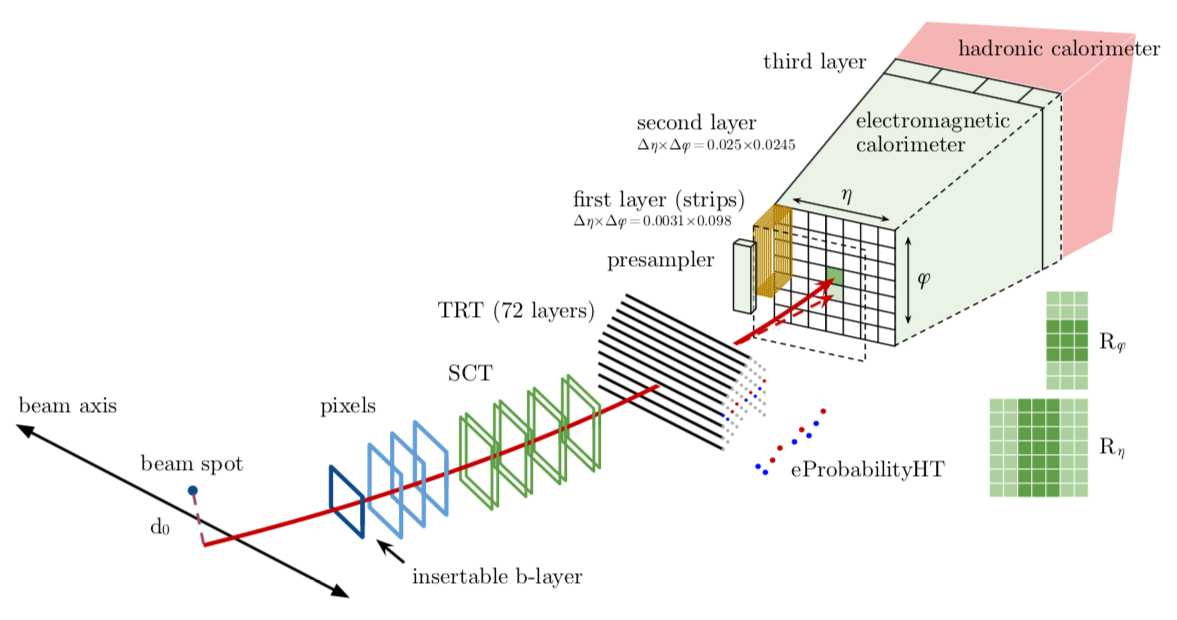
\includegraphics[width=0.9\textwidth]{figures/chapter3/egamma/egamma_lh_input_desc}
        \caption{
        }
        \label{fig:egamma_lh_input_desc}
    \end{center}
\end{figure}

The electron LH is based on the products for the signal and background probability density
functions (PDFs) associated with the set of inputs in Table~\ref{tab:egamma_lh_inputs}:

\begin{align}
    L_{S\,(B)}(\mathbf{x}) = \prod\limits_{i=1}^n P_{S\,(B),i} (x_i),
    \label{eq:egamma_lh}
\end{align}
where $\mathbf{x}$ is the vector of quantities listed in Table~\ref{tab:egamma_lh_inputs} and
the $P_{S\,(B),i}(x_i)$ are the values of the PDF for quantity $i$ at value $x_i$ for the
signal ($S$) and background ($B$).
The likelihoods are built using simulation and the signal is composed of samples of prompt electrons
and the background is built from a combination of jets that mimic the signature of
prompt electrons, electrons from photon conversions, and non-prompt electrons from the decay
of hadrons containing heavy-flavours~\cite{Aad:2019tso}.
The final electron LH discriminant, shown in Figure~\ref{fig:egamma_lh_discriminant}, is based on a transformed version of the ratio,
\begin{align}
    d_L = \frac{L_S}{L_S + L_B},
    \label{eq:egamma_lh_disc}
\end{align}
where the transformation acts to spread $d_L$ to values not bounded by $0$ and $1$,
motivated by the need to have well-defined working points based on selections on $d_L$.

There are four such fixed values of the final LH discriminant that are used to define
four working points corresponding to increasing thresholds on the final LH discriminant:
\textsc{VeryLoose}, \textsc{Loose}, \textsc{Medium}, and \textsc{Tight}.
The efficiencies to identifiy prompt electron candidates are measured using samples of $Z\rightarrow ee$ and
$J/\psi \rightarrow ee$ following a tag-and-probe approach.
They are found, for electron candidates with $E_T > 40\,\GeV$,
to be 93\%, 88\%, and 80\% for the \textsc{Loose}, \textsc{Medium}, and \textsc{Tight} working points, respectively~\cite{Aad:2019tso}.

\begin{figure}[!htb]
    \begin{center}
    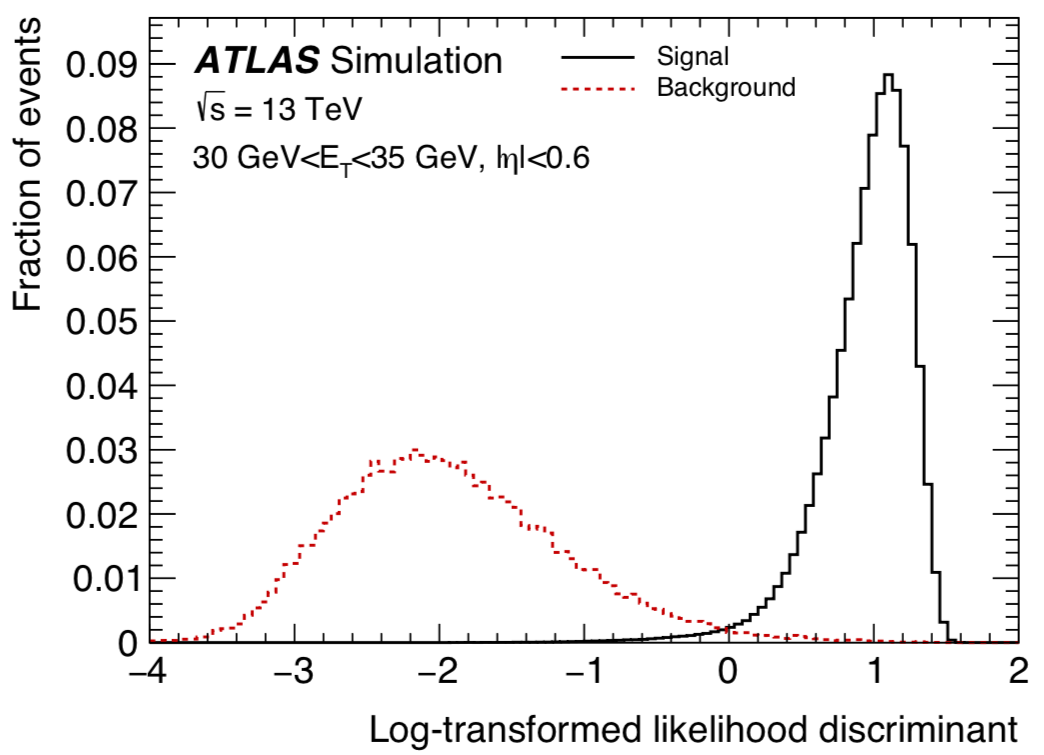
\includegraphics[width=0.7\textwidth]{figures/chapter3/egamma/egamma_lh_discriminant}
    \caption{
        Transformed LH-based electron identification discrimiant for electron candidates
        with $30\,\GeV < E_T < 35\,\GeV$ and $\lvert \eta \rvert < 0.6$.
        From Ref.~\cite{Aad:2019tso}.
    }
    \label{fig:egamma_lh_discriminant}
    \end{center}
\end{figure}

\begin{table}[!htb]
    \caption{
        Variables used as input to construct the electron identification likelihood.
        From Ref.~\cite{Aad:2019tso}.
    }
    \label{tab:egamma_lh_inputs}
    \begin{scriptsize}
    \begin{center}
    \begin{tabularx}{\textwidth}{|X|l|X|}
    \hline
    \hline
    \textbf{Input Type} & \textbf{Name} & \textbf{Description} \\
    \hline
    \multirow{2}{*}{Hadronic Leakage} & $R_{\text{had1}}$ & Ratio of $E_T$ in the first layer of the hadronic calorimeter to $E_T$ of the EM cluster \\
    \cline{2-3}
                & $R_{\text{had}}$ & Ratio of $E_T$ in the hadronic calorimeter to $E_T$ of the EM cluster \\
    \hline
    \multirow{1}{*}{Third layer of EM calorimeter} & $f_3$ & Ratio of the energy in the third layer to the total energy in the
            EM calorimeter. Only used for $E_T<30\,\GeV$  and $\lvert \eta \rvert \le 2.37$. \\
    \hline
    \multirow{3}{*}{Second layer of EM calorimter} & $w_{\eta 2}$ & Lateral shower width,
            \begin{small}$\sqrt{(\sum E_i \eta_i^2) / (\sum E_i) - ((\sum E_i \eta_i) / (\sum E_i))^2}$\end{small},
            where $E_i$ is the energy and $\eta_i$ is the pseudorapidity of cell $i$ and the sum
            is calculated within a window of $3\times5$ cells centered at the electron cluster position. \\ \cline{2-3}
            & $R_{\phi}$ & Ratio of the energy in $3\times 3$ cells over the energy in $3\times7$ cells
            centered at the electron cluster position. \\ \cline{2-3}
            & $R_{\eta}$ & Ratio of the energy in $3\times 7$ cells over the energy in $7\times7$ cells
            centered at the electron cluster position. \\ \cline{2-3}
    \hline
    \multirow{3}{*}{First layer of EM calorimeter} & $w_{stot}$ & Shower width,
            \begin{small} $\sqrt{ (\sum E_i(i - i_{\text{max}})^2)/(\sum E_i)}$ \end{small}, where $i$ runs
            over all strips in a window of $\Delta \eta \times \Delta \phi \approx 0.0625 \times 0.2$,
            corresponding typically to 20 strips in $\eta$, and $i_{\text{max}}$ is the index of the
            highest-energy strip. Used only for $E_T > 150\,\GeV$.\\ \cline{2-3}
            & $E_{\text{ratio}}$ & Ratio of the energy difference between the maximum energy deposit and the energy deposit
            in a secondary maximum in the cluster to the sum of these energies. \\ \cline{2-3}
            & $f_1$ & Ratio of the energy in the first layer to the total energy in the EM calorimeter.\\
    \hline
    \multirow{6}{*}{Track conditions} & $n_{\text{Blayer}}$ & Number of hits in the innermost pixel layer. \\ \cline{2-3}
            & $n_{\text{Pixel}}$ & Number of hits in the pixel detector. \\ \cline{2-3}
            & $n_{\text{Si}}$ & Total number of hits in the pixel and SCT detectors.\\ \cline{2-3}
            & $d_0$ & Transverse impact parameter relative to the beam-spot. \\ \cline{2-3}
            & $\lvert d_0 / \sigma(d_0) \rvert$ & Significance of transverse impact parameter defined as
            the ratio of $d_0$ to its uncertainty. \\ \cline{2-3}
            & $\Delta p / p$ &  Momentum lost by the track between the perigee and the last measurement point
            divided by the momentum at perigee. \\
    \hline
    \multirow{1}{*}{TRT} & eProbabilityHT & Likelihood probability based on transition radiation in the TRT. \\
    \hline
    \multirow{3}{*}{Track-cluster matching} & $\Delta \eta_1$  & $\Delta \eta$ between the cluster position in the first layer
            and the extrapolated track. \\ \cline{2-3}
            & $\Delta \phi_{\text{res}}$ & $\Delta \phi$ between the cluster position in the second layer of the EM calorimeter
            and the momentum-rescaled track, extrapolated from the perigee, times the charge $q$. \\ \cline{2-3}
            & $E/p$ & Ratio of the cluster energy to the track momentum. Used for $E_T>150\,\GeV$.\\
    \hline
    \hline
    \end{tabularx}
    \end{center}
    \end{scriptsize}
\end{table}

\FloatBarrier

\begin{figure}[!htb]
    \begin{center}
        \raisebox{1.35cm}{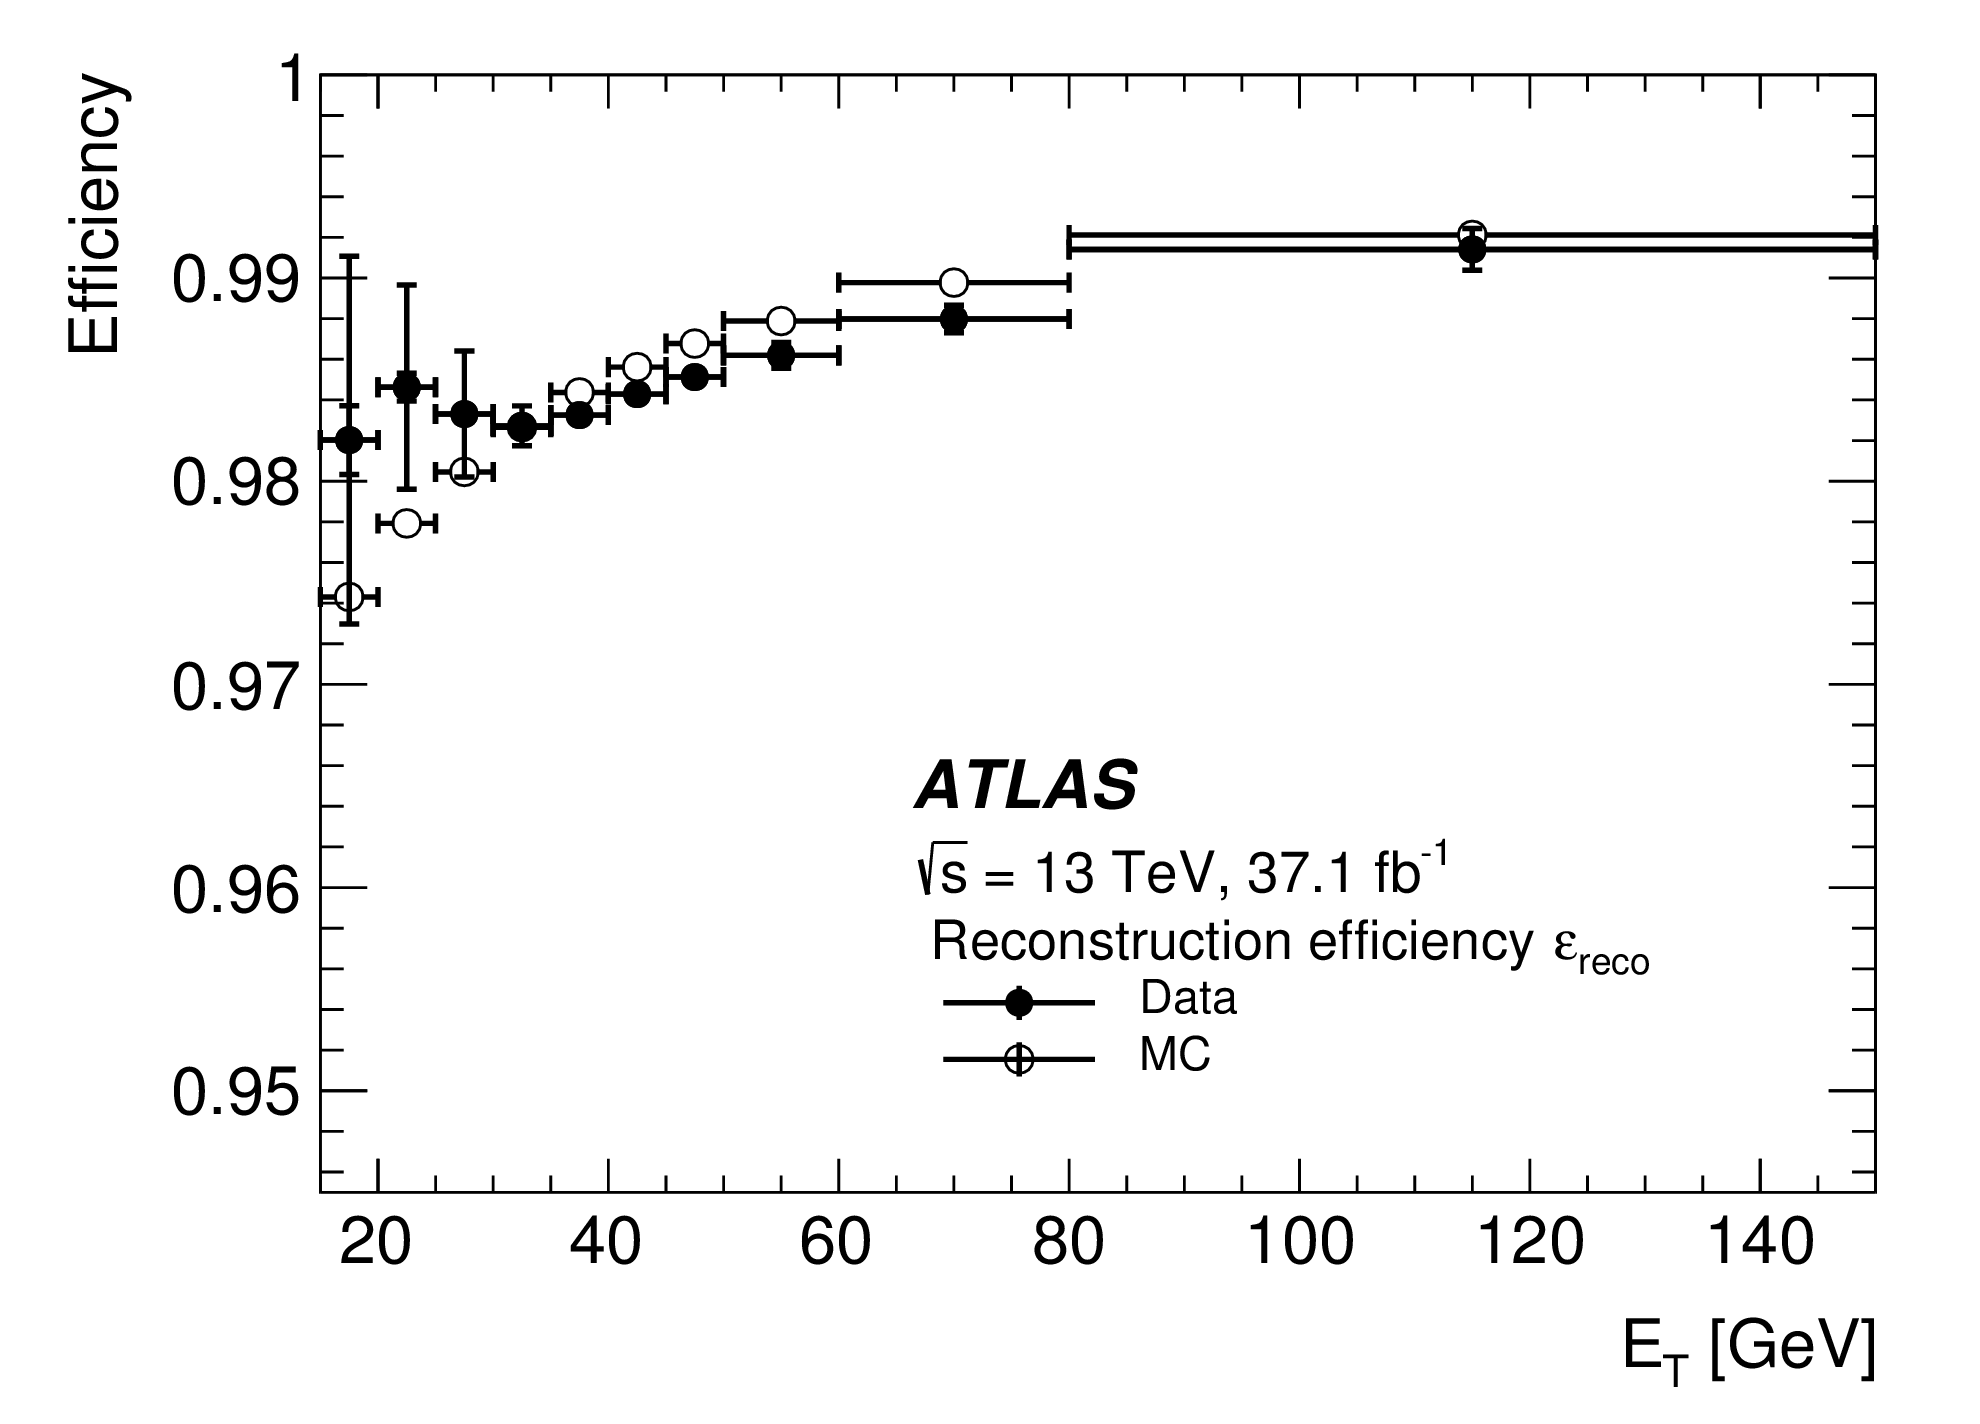
\includegraphics[width=0.48\textwidth]{figures/chapter3/egamma/egamma_reco_eff_Et}}
        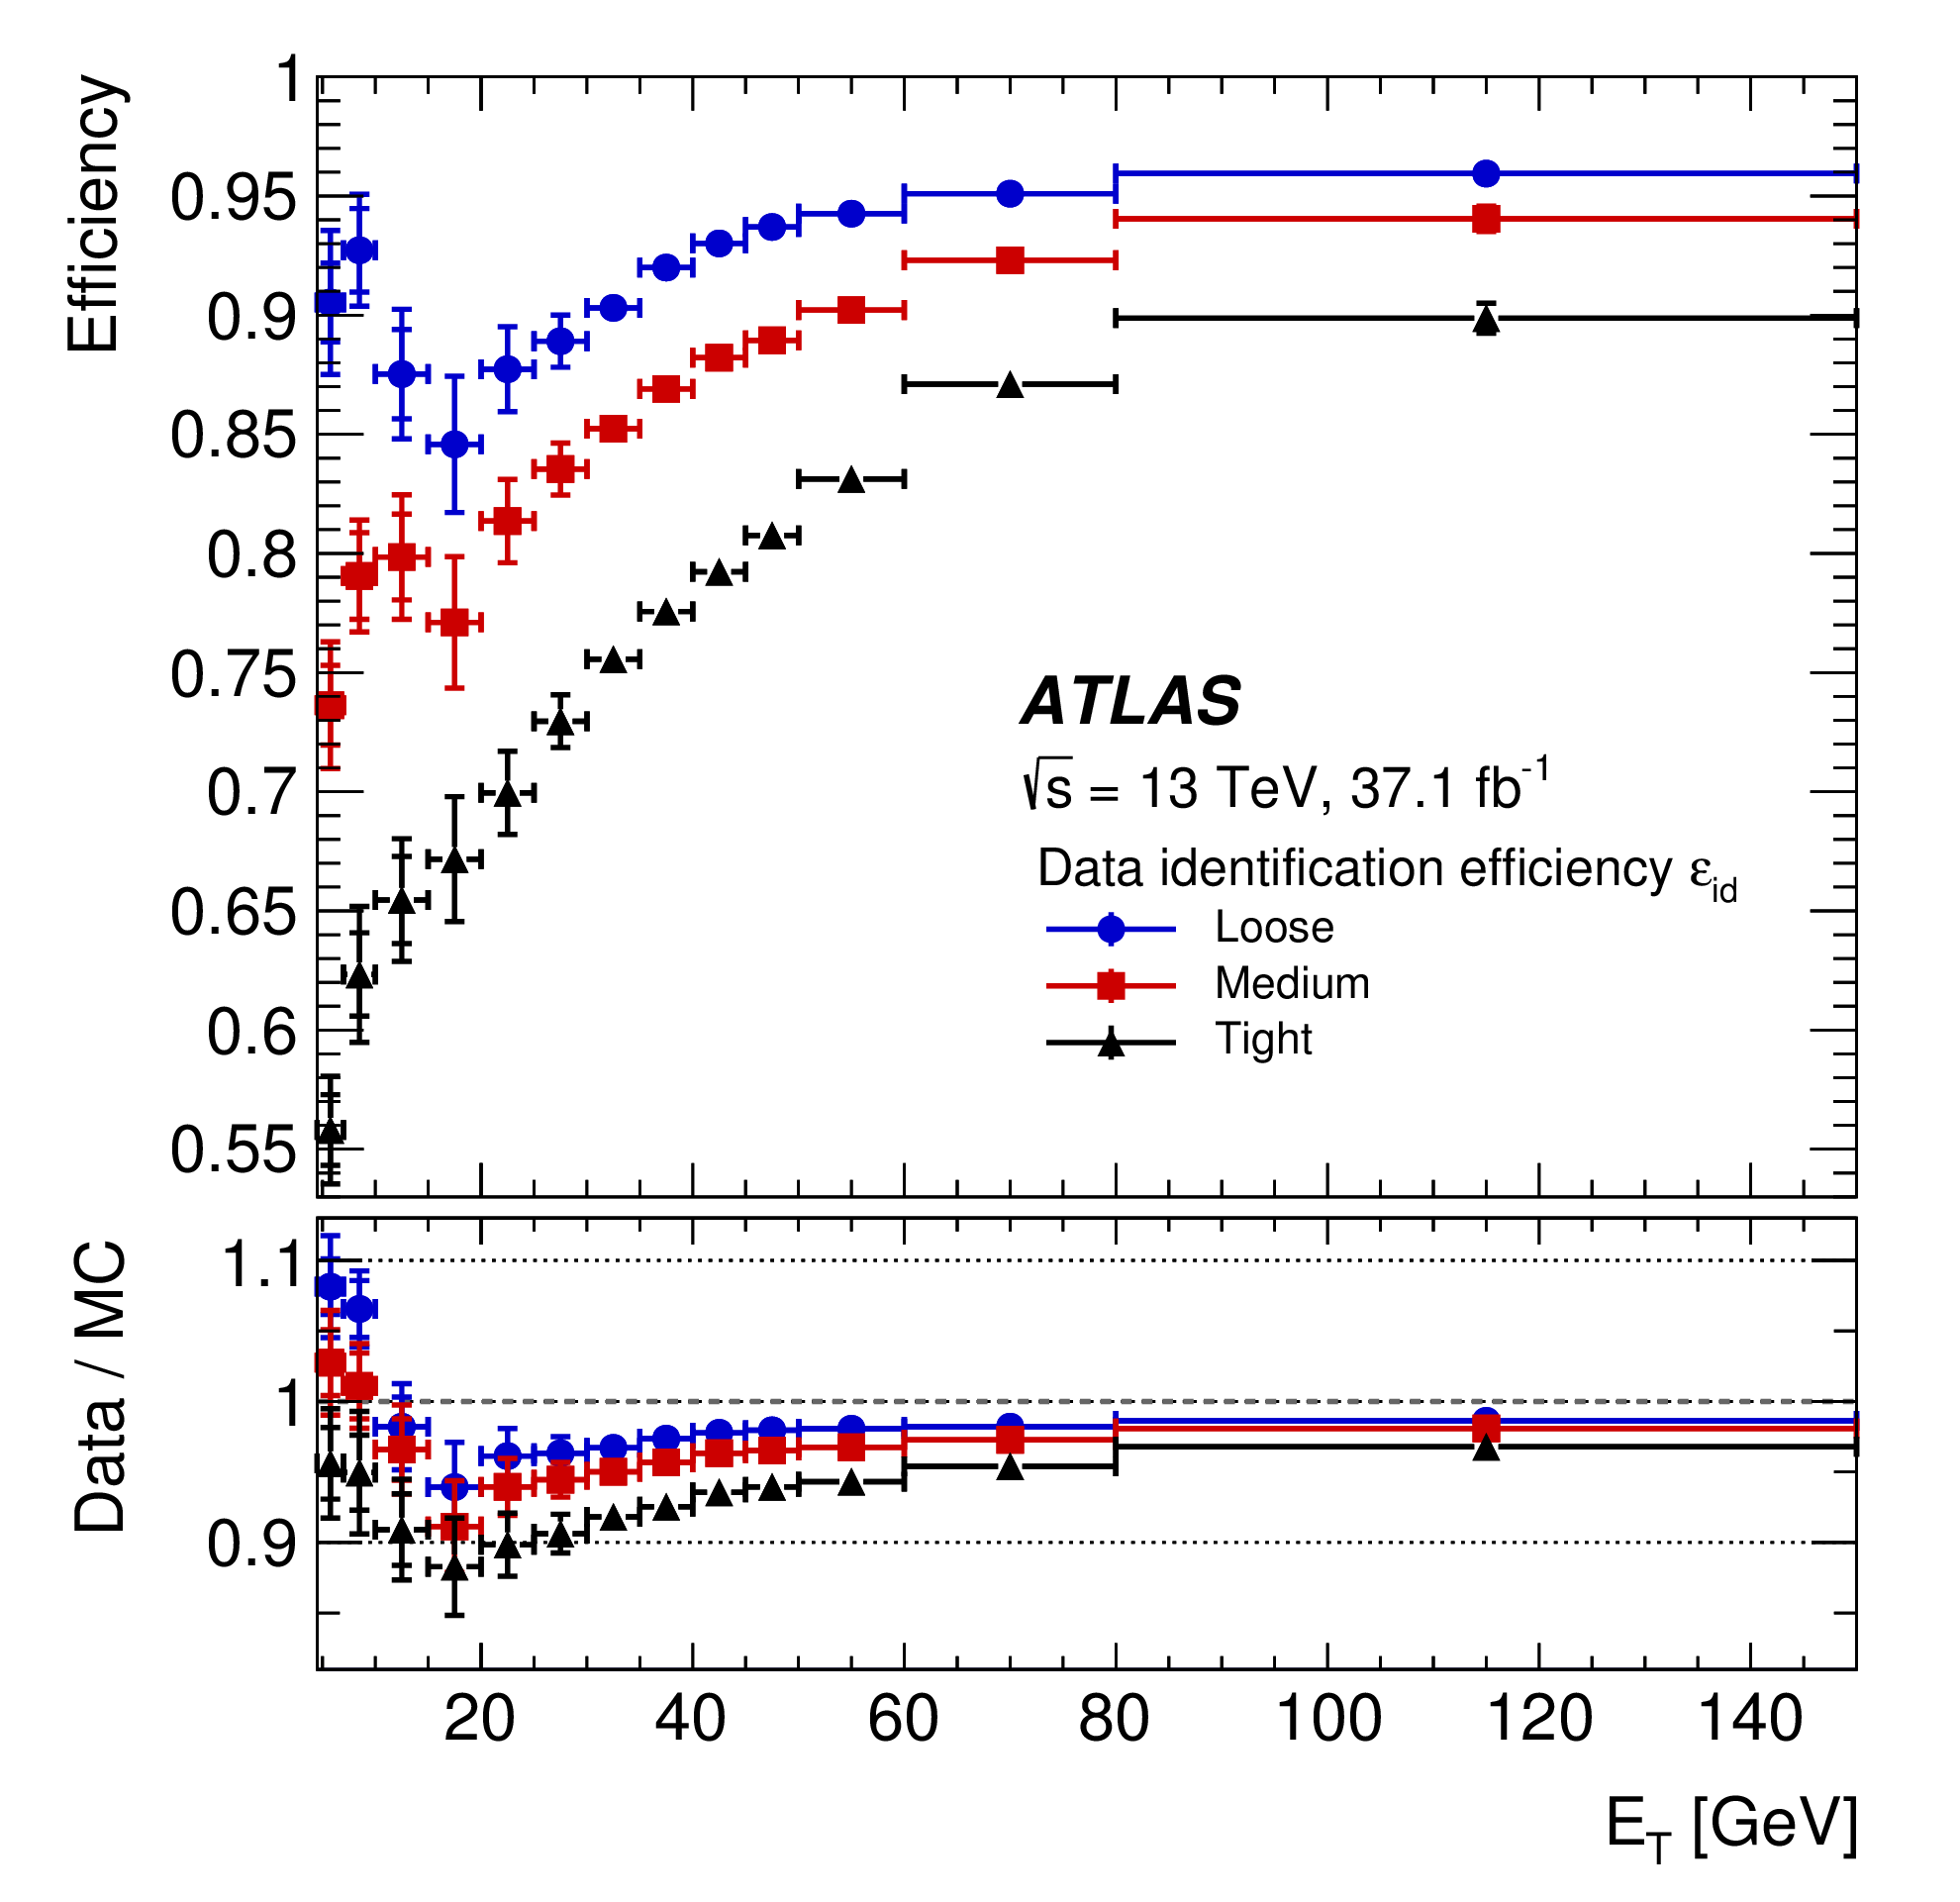
\includegraphics[width=0.48\textwidth]{figures/chapter3/egamma/egamma_id_eff_Et}
        \caption{
            {\color{red}{2015-2016}}
            \textit{Left}: Electron candidate reconstruction efficiency, measured in simulation and in data, as
                a function of the candidate $E_T$.
            \textit{Right}: Electron identification efficiency measured in data, as a function of electron $E_T$,
                for the three standard LH identification working points \textsc{Loose} (blue), \textsc{Medium} (red), and \textsc{Tight} (black).
                The lower panel shows the ratio of the efficiency measured in data over that measured in simulation.
        }
        \label{fig:egamma_eff_Et}
    \end{center}
\end{figure}

\subsection{Muons}
\label{sec:muons}

\subsubsection{Muon Reconstruction}
\label{sec:muon_reco}

The reconstruction of muon candidates is performed by combining the tracking
capabilities of the ID and the MS~\cite{Aad:2016jkr}.
Muon reconstruction first starts with the independent reconstruction of
charged-particle tracks within the ID and the MS.
The independently formed tracks are subsequently combined to form a complete
track representing the traversal of a muon through the full detector.
The muon track in the ID is reconstructed like any other charged-particle track (Section~\ref{sec:tracks_and_vertices}).

Muon reconstruction within the MS starts with a pattern finding phase, looking for
hit patterns each of the muon chambers to then form track segments.
The track segments between different MS layers are then fit together to form muon track candidates.
At least two matching track segments are required in order to build a muon
track candidate, except in the transition region between the barrel and end-cap where
single track-segment candidates can be used.
Once a muon track candidate is formed from the combined segments, a global $\chi^2$ fit is
performed to improve the association of hits to each muon candidate.
The $\chi^2$ is repeated several times, removing outlying hits as necessary, until a
threshold is met for all associated hits.

There are several algorithms used to combine the muon track candidates in the ID and MS, each
using different sets of information related to the ID, MS, and calorimeters.
At the time of the current work, there are four standard combination algorithms used
each based on the subdetectors used in their construction:

\begin{itemize}
    \item{\textbf{Combined Muon (CB)}} This type of muon is formed with a global refit using all muon track candidate hits
        in the ID and the MS. Hits may be added or removed from the MS track candidate during the refit.
        Muons are reconstructed following an outside-in pattern recognition algorithm, in which the
        muon is first reconstructed in the MS and extrapolated inwards to the ID hits.
        A complementary, albeit non-standard, inside-out algorithm also exists.
    \item{\textbf{Segment-tagged Muon (ST)}} An ID track is classified as a muon if, once extrapolated to the MS,
        it is associated with at least one local track segment in the MDT or CSC chambers. Segment-tagged muons
        are used when a muon candidate crosses only one layer of the MS chambers, either because of their
        low \pT~or because they fall into un-instrumented regions of the MS.
    \item{\textbf{Calorimeter-tagged Muon (CT)}} An ID track is classified as a muon if it is matched to an
        energy deposit in the caloriemter that is compatible with a minimum ionising particle.
        Calorimter-tagged muons have the lowest purity, but recover acceptance in regions of the MS
        that are only partially instrumented to allow for cabling and services to the calorimeter and ID systems,
        particularly in the region $\lvert \eta \rvert < 0.1$.
    \item{\textbf{Extrapolated Muon (ME)}} This type of muon is based only on the track candidates formed in the MS
        and a loose requirement that the track candidate be pointing back towards the IP.
        Extrapolated muons are mainly used to extend the acceptance of muon reconstruction into the region
        $2.5 < \lvert \eta \rvert < 2.7$ that is not covered by the ID acceptance.
\end{itemize}

\subsubsection{Muon Identification}
\label{sec:muon_id}

Muon identification refers to the act of applying aditional quality criteria on
the reconstructed muon candidates in order to mainly suppress contamination from
background sources that mimic muon signatures, such as pion and kaon decays, 
while ensuring high rates for the acceptance of prompt muons.
There are three standard muon identification working points in ATLAS, each
a subset of the previous one, and are referred to as the \textsc{Loose},
\textsc{Medium}, and \textsc{Tight} muon identification working points.
\textsc{Medium} muons are the default in ATLAS analyses and can only be composed
of CB and ME muons.
As all muons used in the present thesis are \textsc{Medium} muons, only this
identification working point will be described in detail.

Reconstructed muon candidates originating from non-prompt sources such
as in-flight decays of charged hadrons in the ID, are often characterised by the
presence of a `kink' in the reconstructed muon's track. It is therefore
expected that the independent momentum measurements made in the ID and MS may
be incompatible for non-prompt sources of muon candidates.
The muon identification criteria, then, make use of quantities
that relate the ID and MS muon track candidates.
These quantities are described in Table~\ref{tab:muon_id_vars}.
\textsc{Medium} muons have a rather loose selection on the compatibility between
the ID and MS momentum measurements and, with respect to those quantities in Table~\ref{tab:muon_id_vars},
are only required to have a $q/p$ significance less than 7.
On top of requirements on those quantities described in Table~\ref{tab:muon_id_vars},
the muon identification working points place
additional requirements on the number and type of hits in the ID and MS.
All identification working points require, in the ID, that there be at least 1 hit
in the pixel subdetector, at least 5 hits in the SCT subdetector, less
than 3 silicon holes,\footnote{A missing hit is considered a `hole' only
if it falls between hits successfully assigned to a given track.}
and at least 10\% of the TRT hits originally assigned to the muon track candidate exist
after the combined reconstruction.
\textsc{Medium} muons further require that the CB muons have at least 3 hits in at least
two MDT layers, except in $\lvert \eta \rvert < 0.1$ where tracks with at least one MDT layer but no more
than one MDT hole are allowed. The ME \text{Medium} muons are required to have at least
3 MDT or CSC layer hits, and are employed only in $2.5 < \lvert \eta \rvert < 2.7$.


\begin{table}[!htb]
    \begin{center}
        \begin{tabularx}{\textwidth}{l|X|X}
        \hline
        \hline
        \textbf{Quantity Name} & \textbf{Measurement} & \textbf{Description} \\
        \hline
        $q/p$ significance & $\lvert (q/p)^{\text{ID}} - (q/p)^{\text{MS}} \rvert / \sqrt{ \sigma_{p_T}^{\text{MS}} + \sigma_{p_T}^{\text{ID}}}$ &
                Absolute value of the difference between the ratio of the charge and momentum of the muon candidates measured in the ID and MS,
                divided by the quadrature sum of the corresponding uncertainties. \\
        \hline
        $\rho^{\prime}$ & $\lvert p_T^{\text{MS}} - p_T^{\text{ID}} \rvert / p_T^{\text{Combined}}$ &
                Absolute value of the difference between the transverse momentum measurements in the ID and the MS,
                divided by that of the combined muon candidate. \\
        \hline
        $\chi^2_{\text{norm}}$ & -- & Normalized $\chi^2$ of the combined muon track fit \\
        \hline
        \hline
        \end{tabularx}
    \end{center}
    \caption{
    }
    \label{tab:muon_id_vars}
\end{table}

\begin{figure}[!htb]
    \begin{center}
        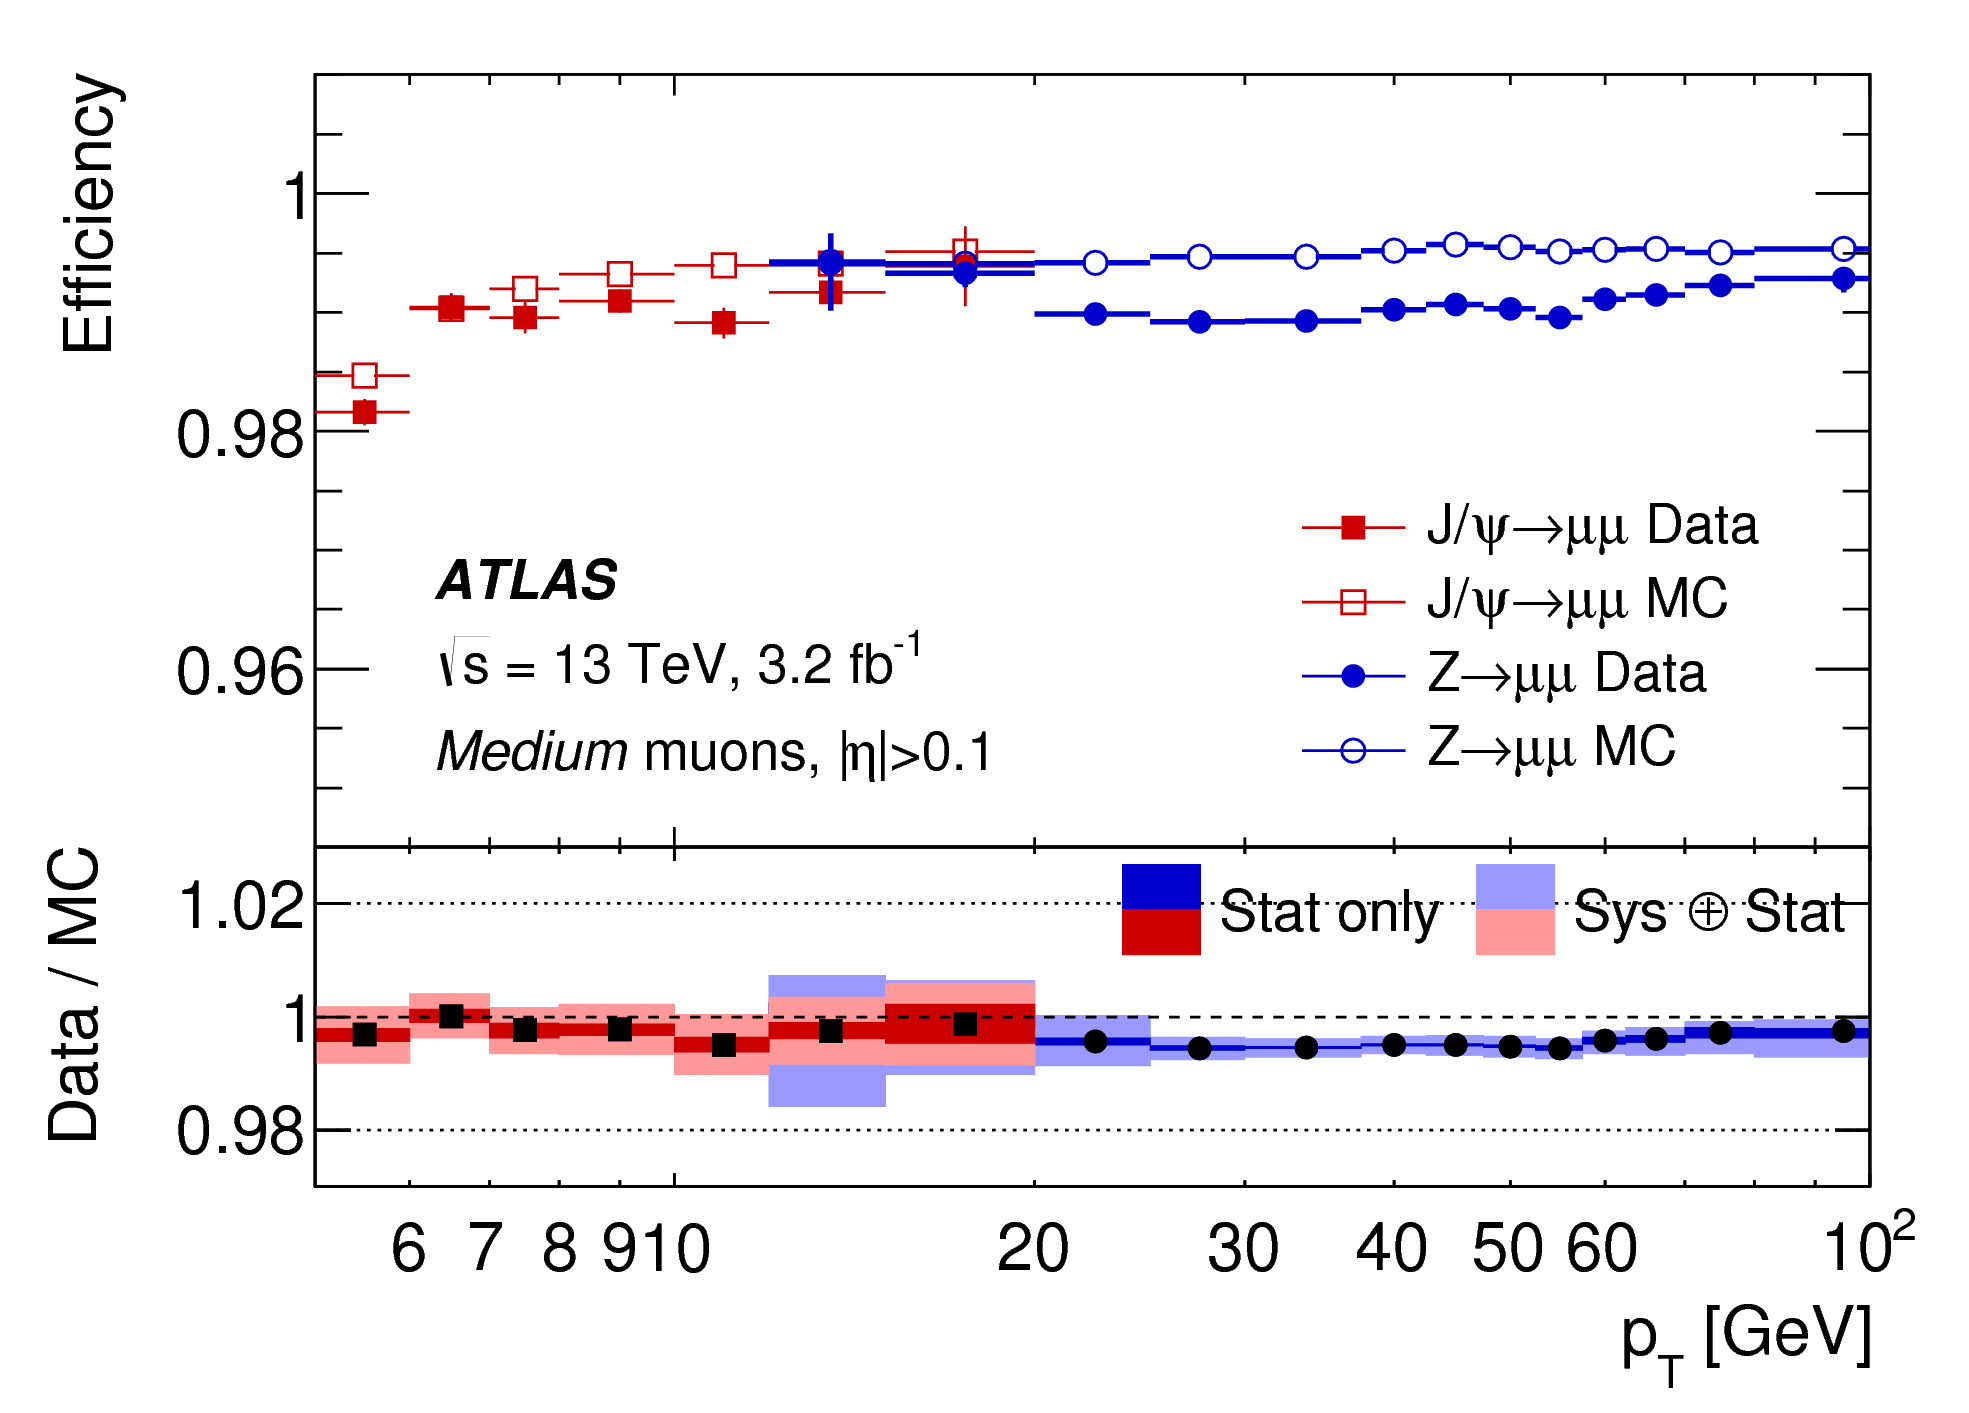
\includegraphics[width=0.7\textwidth]{figures/chapter3/muon/muon_reco_eff_medium}
        \caption{
            From Ref.~\cite{Aad:2016jkr}.
        }
        \label{fig:muon_reco_eff}
    \end{center}
\end{figure}

\FloatBarrier

